\section{Auswertung}
\label{sec:Auswertung}

\subsection{Spektrum des \textsuperscript{137}Cs-Strahlers}

Das aufgenommene Spektrum des \textsuperscript{137}Cs-Strahlers ist in Abbildung
\ref{fig:verlauf} dargestellt.

\begin{figure}[H]
  \centering
  \includegraphics{verlauf.pdf}
  \caption{Aufgenommenes Spektrum des \textsuperscript{137}Cs-Strahlers.}
  \label{fig:verlauf}
\end{figure}

Eindeutig zu erkennen ist das Compton-Kontinuum im Bereich kleiner Channel (Energien).
Im Bereich um Channel $90$ ist dann die Compton-Kante zu finden. In diesem Bereich
fällt die Anzahl an Counts noch einmal eindeutig ab. Der eigentliche Peak der $\gamma$-Strahlung der Caesium-Quelle
ist dann in einem Bereich um Channel 127 zu erkennen. Dieser hat eine gewisse Breite,
weshalb im Folgenden die Zählraten durch Integration über eben diesen Bereich im
entsprechenden Spektrum ermittelt werden.

\subsection{Abschwächung des Aluminiumwürfels}
Die gemessenen Counts $N$ des ersten Würfels, sowie die daraus resultierenden Zählraten  $I_{0,\mathrm{i}}$ bei einer Messung
über $\SI{20}{\second}$ sind in Tabelle \ref{tab:w1} dargestellt.

\begin{table}[H]
  \centering
  \caption{Zählrate in Abhängigkeit der Projektion bei einer Messdauer von $\SI{100}{\second}$ }
  \label{tab:w1}
  \begin{tabular}{c c c}
    \toprule
    Projektion & $N$ & $I_{0,\mathrm{i}} / \frac{1}{\symup{s}}$  \\
    \midrule
        $I_1$    & $\SI{16161(152)}{}$ & $\SI{161.61(152)}{}$    \\
        $I_2$    & $\SI{16165(151)}{}$ & $\SI{161.65(151)}{}$    \\
        $I_3$    & $\SI{16218(151)}{}$ & $\SI{162.18(151)}{}$    \\
        $I_4$    & $\SI{15596(151)}{}$ & $\SI{155.96(151)}{}$    \\
        $I_5$    & $\SI{15662(151)}{}$ & $\SI{156.62(151)}{}$    \\
        $I_6$    & $\SI{15899(152)}{}$ & $\SI{158.99(152)}{}$    \\
        $I_7$    & $\SI{15997(153)}{}$ & $\SI{159.97(153)}{}$    \\
        $I_8$    & $\SI{16187(152)}{}$ & $\SI{161.87(152)}{}$    \\
        $I_9$    & $\SI{16213(153)}{}$ & $\SI{162.13(153)}{}$    \\
        $I_{10}$ & $\SI{15509(151)}{}$ & $\SI{155.09(151)}{}$   \\
        $I_{11}$ & $\SI{15725(151)}{}$ & $\SI{157.25(151)}{}$    \\
        $I_{12}$ & $\SI{15605(152)}{}$ & $\SI{156.05(152)}{}$    \\
    \bottomrule
  \end{tabular}
\end{table}

Die $I_{0,\mathrm{i}}$ sind für die weiteren Berechnungen die Ausgangszählraten,
da alle anderen Würfel von einem Aluminiumwürfel ummantelt sind.


\subsection{Abschwächungskoeffizienten des zweiten Würfels}

Die vier gemessenen Zählraten $N_\symup{i}$ sind mit ihrer zugehörigen Projektion in Tabelle
\ref{tab:w2} aufgeführt. Die Zuordnung der Projektionen entspricht derjenigen aus dem
vorherigen Abschnitt. Die Messdauer beträgt $\SI{300}{\second}$.

\begin{table}[H]
  \centering
  \caption{Zählraten des zweiten Würfels in Abhängigkeit der Projektion bei einer Messdauer von $\SI{300}{\second}$ }
  \label{tab:w2}
  \begin{tabular}{c c}
    \toprule
    Projektion & $N_{\mathrm{i}} / \frac{1}{\symup{s}}$   \\
    \midrule
        $I_1$    & $\SI{25.56(36)}{}$ \\
        $I_2$    & $\SI{24.04(36)}{}$ \\
        $I_5$    & $\SI{17.13(31)}{}$ \\
        $I_6$    & $\SI{18.81(32)}{}$ \\
    \bottomrule
  \end{tabular}
\end{table}

Daraus lassen sich nach Gleichung \ref{eqn:mu} die Absorptionskoeffizienten bestimmen.
Die Kantenlänge des inneren Würfels beträgt $\SI{3}{\centi\meter}$.
Die Ergebnisse sind in Tabelle \ref{tab:mu2} aufgeführt.

\begin{table}[H]
  \centering
  \caption{Berechnete Absorptionskoeffizienten des zweiten Würfels in Abhängigkeit der Projektion}
  \label{tab:mu2}
  \begin{tabular}{c c}
    \toprule
    Projektion & $\mu_{\mathrm{i}} / \frac{1}{\symup{s}}$   \\
    \midrule
        $I_1$    & $\SI{0.615(6)}{}$ \\
        $I_2$    & $\SI{0.635(6)}{}$ \\
        $I_5$    & $\SI{0.522(5)}{}$ \\
        $I_6$    & $\SI{0.755(7)}{}$ \\
    \bottomrule
  \end{tabular}
\end{table}

Es ergibt sich ein Mittelwert von:
\begin{equation*}
  \bar\mu_2 = \SI{0.632(3)}{1\per\centi\meter}
\end{equation*}


\subsection{Abschwächungskoeffizienten des dritten Würfels}

Die vier gemessenen Zählraten $N_\symup{i}$ sind mit ihrer zugehörigen Projektion in Tabelle
\ref{tab:w3} aufgeführt. Die Zuordnung der Projektionen entspricht derjenigen aus dem
vorherigen Abschnitt. Die Messdauer beträgt $\SI{300}{\second}$.

\begin{table}[H]
  \centering
  \caption{Zählraten des dritten Würfels in Abhängigkeit der Projektion bei einer Messdauer von $\SI{300}{\second}$ }
  \label{tab:w3}
  \begin{tabular}{c c}
    \toprule
    Projektion & $N_{\mathrm{i}} / \frac{1}{\symup{s}}$   \\
    \midrule
        $I_1$    & $\SI{109.66(75)}{}$ \\
        $I_2$    & $\SI{107.91(75)}{}$ \\
        $I_5$    & $\SI{102.99(73)}{}$ \\
        $I_6$    & $\SI{97.85(71)}{}$ \\
    \bottomrule
  \end{tabular}
\end{table}

Daraus lassen sich wieder nach Gleichung \ref{eqn:mu} die Absorptionskoeffizienten bestimmen.
Die Kantenlänge des inneren Würfels beträgt auch hier $\SI{3}{\centi\meter}$.
Die Ergebnisse sind in Tabelle \ref{tab:mu3} aufgeführt.

\begin{table}[H]
  \centering
  \caption{Berechnete Absorptionskoeffizienten des dritten Würfels in Abhängigkeit der Projektion}
  \label{tab:mu3}
  \begin{tabular}{c c}
    \toprule
    Projektion & $\mu_{\mathrm{i}} / \frac{1}{\symup{s}}$   \\
    \midrule
        $I_1$    & $\SI{0.129(4)}{}$ \\
        $I_2$    & $\SI{0.135(4)}{}$ \\
        $I_5$    & $\SI{0.099(3)}{}$ \\
        $I_6$    & $\SI{0.172(4)}{}$ \\
    \bottomrule
  \end{tabular}
\end{table}

Es ergibt sich ein Mittelwert von:
\begin{equation*}
  \bar\mu_3 = \SI{0.134(2)}{1\per\centi\meter}
\end{equation*}


\subsection{Abschwächungskoeffizienten des vierten Würfels}
Die Abschwächungskoeffizienten der einzelenen Materialien werden mit Gleichung (3) bestimmt. Die Dicke
der Elementarwürfel beträgt dabei $d=\SI{1}{\centi\meter}$. In Tabelle (?) werden die gemessenen Zählraten und
die daraus berechneten Abschwächungskoeffizienten dargestellt.

\begin{table}[H]
  \centering
  \caption{Zählrate in Abhängigkeit der Projektion bei einer Messdauer von $\SI{300}{\second}$ und und Abschwächungskoeffizienten }
  \label{tab:Parameter}
  \begin{tabular}{c c c | c c}
    \toprule
    Projektion & $N$ & Fehler & $\mu$ & Fehler   \\
    \midrule
        $I_1$    & 16161 & 152 & &    \\
        $I_2$    & 16165 & 151 & &    \\
        $I_3$    & 16218 & 151 & &    \\
        $I_4$    & 15596 & 151 & &    \\
        $I_5$    & 15662 & 151 & &    \\
        $I_6$    & 15899 & 152 & &    \\
        $I_7$    & 15997 & 153 & &    \\
        $I_8$    & 16187 & 152 & &    \\
        $I_9$    & 16213 & 153 & &    \\
        $I_{10}$ & 15509 & 151 & &   \\
        $I_{11}$ & 15725 & 151 & &    \\
        $I_{12}$ & 15605 & 152 & &    \\
    \bottomrule
  \end{tabular}
\end{table}


\begin{figure}
  \centering
  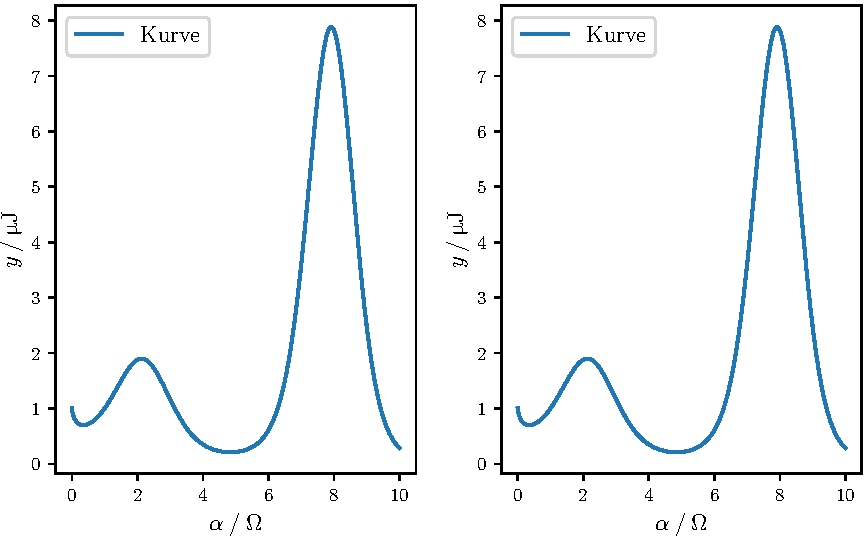
\includegraphics{plot.pdf}
  \caption{Plot.}
  \label{fig:plot}
\end{figure}
